\label{Chapter7} % For referencing the chapter elsewhere, use \ref{Chapter7} 
\chapter{Outlook} % Main chapter title


The first physics run started in November 2017 with several months of fine tuning the muon beam injection and storage prior to data taking beginning. Two physics runs have so far been completed achieving just over 4 times the BNL statistics as shown in figure 8.1. The experiment is currently carrying out upgrades for the third physics run which will begin around October 2019 and aims to reach 10 times the BNL statistics. 

The straw tracking detectors have proved themselves to be extremely valuable and have worked extremely stably throughout data taking, providing real time beam profile measurements. The ability to give real time measurements of the muon beam distribution has enabled any problems with the beam storage to be quickly identified and fixed. 

The target dataset for the Fermilab muon g-2 experiment is 21 time the BNL dataset. The final dataset will be the most precise measurement of $a_{\mu}$ ever measured. With the aim of reducing the uncertainties of the measurement by a factor of four compared to the BNL experiment. With this improvement in precision, if the $a_{\mu}$ value remains unchanged then this would give evidence for previously unknown physical interaction by giving $\sim$ 7$\sigma$ discrepancy between the experimental measurement and the SM calculation.

This thesis has detailed the design, construction and testing of the straw tracking modules carried out in the cleanrooms of the University of Liverpool. This encompassed a large portion of my PhD, spending the first two and a half years working on this and was detailed in chapter 6. The production of 22 tracking modules is completed, with 16 installed in the experimental storage ring and the remainders shipped to Fermilab as spares. The modules installed in the storage ring are running with 99.7$\%$ of the channels. Quality assurance testing proved that the modules work very efficiently at the required operational wire voltage. The modules have proven that the leak rate is below requirements and the straw resolution which was designed to be at least 300 $\mu$m has surpassed that to a value of 95 $\mu$m. So far there has been no major faults with any of the modules and are proving to be one of the most robust piece of hardware of the experiment. This bears testament to the amount of attention to detail and stringent quality assurance testing that went into every step of the construction and testing process.

Using tracking data, I carried out a beam dynamics study. This was to characterise the behaviour of the vertical components of the muon beam throughout the fill. Looking at this behaviour variations in the expected frequencies were observed. This variation needed to be characterised more precisely so that it could be included in the $\omega_{a}$ fit function, and not distort the extracted value of $\omega_{a}$.



\begin{figure}[th]
\centering
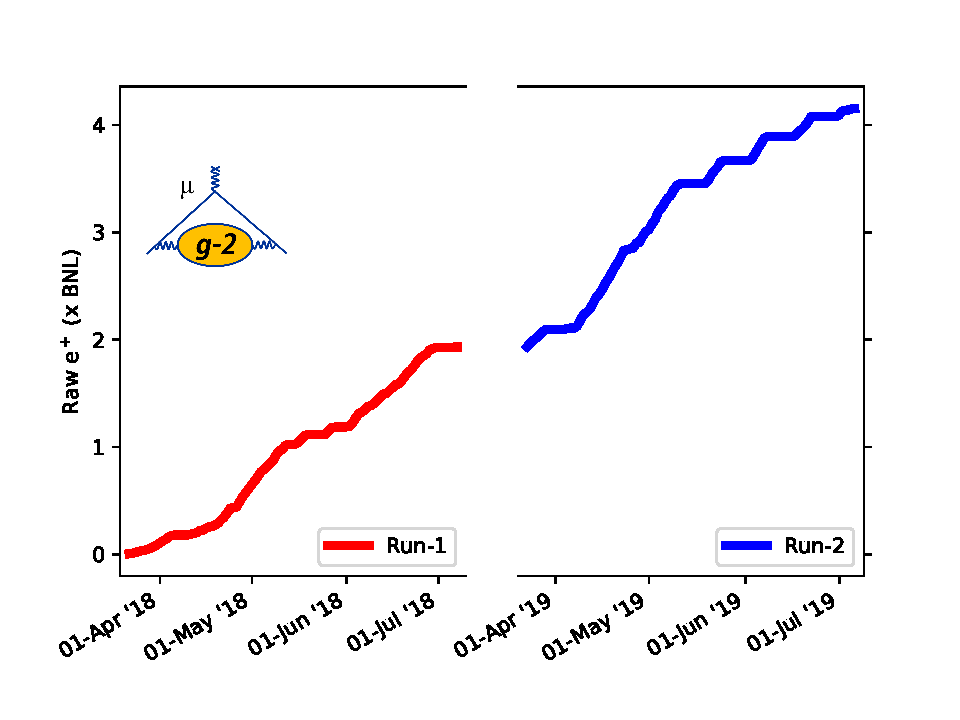
\includegraphics[scale=0.8]{Figures/plot_integrated_ctag.pdf}
\decoRule
\caption{The number of recorded positrons by the calorimeters taken for run 1 and run 2 compared to the BNL dataset. The run 2 dataset pushed the recorded number to just over 4 times the BNL dataset.}
\label{fig:plot_integrated_ctag}
\end{figure}
